\section{Setting, and what we use from Baek's paper}\label{sec:setting}

This section fixes the notation and records the results that the proof uses and does not prove; we call
them \emph{Facts}. Most are results of Baek's paper~\cite{Baek}, quoted in the form in which we use them
and with the numbering of version~1 of the preprint (chapter.section.number). A few printed statements need a
correction, and a few are used for objects slightly more general than those of their printed statements;
each such place is noted with a label E$n$, the number of the correction in the audit that accompanies the
formalization~\cite{Companion}, and Appendix~\ref{app:corrections} lists them. Some corrections come from
the notes of another formalization of Baek's proof~\cite{Cureton}. Three Facts are known to us only through
the formalization, because the printed proof is missing or invalid, or because the statement is not in~\cite{Baek}: \cref{fact:Q}\ref{fact:Q:triple} (E21),
\cref{fact:gerver} (E12, E24) and \cref{fact:height}; they are proved in~\cite{Companion}, and
\cref{sec:formalization} says what that means. The reader who knows~\cite{Baek} can skim this section and
return to it for the notation.

\subsection{Notation and convex bodies}

The plane is $\R^2$, with points $p=(x,y)$, inner product $\ip pq$ and norm $\norm p$; $\abs X$ is the
area (Lebesgue measure) of $X\subset\R^2$. For an angle $t\in\R$ put
\[
  u_t=(\cos t,\sin t),\qquad v_t=(-\sin t,\cos t)=u_{t+\pi/2},
\]
and let $R_t$ be the counterclockwise rotation by $t$. For $c\in\R$ let
$l(t,c)=\{p:\ip p{u_t}=c\}$, $H_-(t,c)=\{p:\ip p{u_t}\le c\}$, $H_+(t,c)=\{p:\ip p{u_t}\ge c\}$, and let
$H^\circ_\pm$ be the open half-planes. The half-plane $H_-(t,c)$ has \emph{normal angle} $t$.

A \emph{convex body} is a nonempty compact convex subset of $\R^2$; it may be a segment or a point. Its
\emph{support function} is $h_K(t)=\max_{p\in K}\ip p{u_t}$, its \emph{supporting line} is
$l_K(t)=l(t,h_K(t))$, and $H_K(t)=H_-(t,h_K(t))$. Then $K=\bigcap_tH_K(t)$, so $h_K$ determines $K$;
$h_{K+w}(t)=h_K(t)+\ip w{u_t}$ and $h_{(1-\lambda)K+\lambda L}=(1-\lambda)h_K+\lambda h_L$ for
Minkowski combinations. The Hausdorff distance is $\dH(K,L)=\sup_t\abs{h_K(t)-h_L(t)}$, and
$K_n\to K$ means $\dH(K_n,K)\to0$. The \emph{edge} of $K$ with normal angle $t$ is the segment
$e_K(t)=K\cap l_K(t)=[v_K^-(t),v_K^+(t)]$, where $v_K^+(t)$ is its endpoint farthest in the
direction $v_t$; it may be a point. For angles $a,b$ with $\sin(b-a)\ne0$ the supporting lines
$l_K(a)$ and $l_K(b)$ meet at
\[
  v_K(a,b)=h_K(a)\,u_a+\frac{h_K(b)-h_K(a)\cos(b-a)}{\sin(b-a)}\,v_a .
\]

\begin{fact}[convex bodies]\label{fact:convex}
Let $K$ be a convex body.
\begin{enumerate}[label=(\alph*)]
\item\label{fact:convex:vertices} $h_K$ has the one-sided derivatives $h_K'(t^\pm)=\ip{v_K^\pm(t)}{v_t}$;
$v_K^+$ is right-continuous and $v_K^-$ left-continuous; $v_K(t,s)\to v_K^+(t)$ as $s\downarrow t$ and
$v_K(s,t)\to v_K^-(t)$ as $s\uparrow t$. \baek{Thm.~2.1.3}
\item\label{fact:convex:sigma} The \emph{surface area measure} $\sigma_K$ is the Lebesgue--Stieltjes measure
on $\R$ of $G_K(t)=\ip{v_K^+(t)}{v_t}+\int_0^th_K$ (formally $\sigma_K=h_K''+h_K$); it is
$2\pi$-periodic. We write $\sigma_K(t)=\sigma_K(\{t\})$. Its atoms are the edge lengths:
$\sigma_K(t)=\abs{e_K(t)}$ and $v_K^+(t)=v_K^-(t)+\sigma_K(t)v_t$. Moreover
$v_K^+(d)-v_K^+(c)=\int_{(c,d]}v_s\dd\sigma_K(s)$ for $c\le d$, and
$\abs K=\tfrac12\int_{[0,2\pi)}h_K\dd\sigma_K$.
\baek{Prop.~2.1.2, Thm.~5.2.2}, \cite[Rem.~5.1.2]{Schneider14}
\item\label{fact:convex:blaschke} Every sequence of convex bodies in a bounded set has a subsequence that
converges to a convex body (Blaschke's selection theorem), and $K\mapsto\abs K$ is continuous for $\dH$.
\cite[Section~1.8, in particular Thm.~1.8.20]{Schneider14}
\end{enumerate}
\end{fact}

Baek's Thm.~2.1.3 states the limits in \ref{fact:convex:vertices}; the formulas for the one-sided derivatives follow from them and
from $\ip{v_K(t,s)}{v_t}=\bigl(h_K(s)-h_K(t)\cos(s-t)\bigr)/\sin(s-t)$, and the printed statement has a misprint (E27).
From \ref{fact:convex:sigma} one reads off, for $a<b$,
\begin{equation}\label{eq:sigma-open}
  \sigma_K\bigl((a,b)\bigr)=\ip{v_K^-(b)}{v_b}-\ip{v_K^+(a)}{v_a}+\int_a^bh_K .
\end{equation}

\subsection{Moving sofas, monotonization, caps and niches}\label{sec:sofas}

The \emph{hallway} is $L=H_L\cup V_L$, the union of its horizontal side $H_L=(-\infty,1]\times[0,1]$
and its vertical side $V_L=[0,1]\times(-\infty,1]$; its inner corner is the origin $O$ and its outer
corner is $(1,1)$.

\begin{definition}[moving sofa]\label{def:sofa}
A \emph{movement} of a set $S\subset\R^2$ is a pair of continuous maps $\theta:[0,1]\to\R$,
$c:[0,1]\to\R^2$ with $\theta(0)=0$ such that the rigid motions $\Phi_s(p)=R_{\theta(s)}p+c(s)$ satisfy
\[
  \Phi_0(S)\subset H_L,\qquad \Phi_s(S)\subset L\ \ (0\le s\le1),\qquad \Phi_1(S)\subset V_L .
\]
Its \emph{rotation angle} is $\omega=-\theta(1)$. A \emph{moving sofa} is a nonempty, closed and
connected set that has a movement; it is a moving sofa \emph{with rotation angle $\omega$} if it has a
movement with that rotation angle.
\end{definition}

This is \baek{Def.~1.1.2}: Baek moves the set along a continuous curve of orientation-preserving
isometries that starts at a translation, and the angle of such a curve lifts to a continuous real
function. A moving sofa is bounded, hence compact: the start and end positions bound it unless $\theta(1)\in\pi/2+2\pi\mathbb Z$, and then a
position in the middle of the movement does (in Lean, \path{isBounded_of_isMovingSofa}). A translate of a moving sofa with
rotation angle $\omega$ is again one. Let $\omega_0=\sec^{-1}(11/5)=\arccos(5/11)=1.0989\ldots$ ($63^\circ$ approximately).

For $\omega\in(0,\pi/2]$ let $H=\R\times[0,1]$ be the horizontal strip, $V_\omega=\{p:0\le\ip p{u_\omega}\le1\}$,
$P_\omega=H\cap V_\omega$ the parallelogram (a strip if $\omega=\pi/2$), and
$F_\omega=\{p:y\ge0,\ \ip p{u_\omega}\ge0\}$ the \emph{fan}. If $\omega<\pi/2$ the two upper sides of
$P_\omega$ meet at $o_\omega=(c_\omega,1)$, $c_\omega=\sec\omega-\tan\omega$, and the two lower sides at $O$.
A moving sofa $S$ with rotation angle $\omega$ is in \emph{standard position} if $h_S(\omega)=h_S(\pi/2)=1$.

\begin{fact}[rotation angle and standard position]\label{fact:angle}
\begin{enumerate}[label=(\alph*)]
\item Every moving sofa $S$ with $\abs S\ge 11/5$ is a moving sofa with some rotation angle
$\omega\in[\omega_0,\pi/2]$. \baek{Thm.~1.5.1}
\item If $S$ is a moving sofa with rotation angle $\omega\in(0,\pi/2]$, some translate $S+v$ is in
standard position, and a moving sofa with rotation angle $\omega$ in standard position
lies in $P_\omega$. \baek{Prop.~1.2.1, Prop.~2.3.1}
\end{enumerate}
\end{fact}

\runin{Supporting hallways.} For a compact set $S$ and an angle $t$ let
\[
  f_{S,t}(p)=R_tp+(h_S(t)-1)u_t+(h_S(t+\pi/2)-1)v_t ,
\]
and let $L_S(t)=f_{S,t}(L)$ be the \emph{supporting hallway} of $S$ at $t$: the translate of $R_tL$
whose two outer walls $a_S(t)=l_S(t)$ and $c_S(t)=l_S(t+\pi/2)$ are supporting lines of $S$. Its inner
corner and outer corner are
\begin{align*}
  \xx_S(t)&=(h_S(t)-1)u_t+(h_S(t+\pi/2)-1)v_t,\\
  \yy_S(t)&=h_S(t)u_t+h_S(t+\pi/2)v_t=\xx_S(t)+u_t+v_t,
\end{align*}
its inner walls lie on the lines $b_S(t)=l(t,h_S(t)-1)$ and $d_S(t)=l(t+\pi/2,h_S(t+\pi/2)-1)$ (the half-lines
from $\xx_S(t)$ in the directions $-v_t$ and $-u_t$ are $\vec b_S(t)$ and $\vec d_S(t)$), and
\begin{align*}
  L_S(t)&=Q_S^+(t)\setminus Q_S^-(t),\qquad
  Q_S^+(t)=H_S(t)\cap H_S(t+\tfrac\pi2),\\
  Q_S^-(t)&=H^\circ_-(t,h_S(t)-1)\cap H^\circ_-(t+\tfrac\pi2,h_S(t+\tfrac\pi2)-1).
\end{align*}
$Q_S^-(t)$ is the open quarter-plane below the inner corner. A moving sofa in standard position lies in
$L_S(t)$ for every $t\in[0,\omega]$, and the \emph{monotonization} of $S$ is
\[
  \cI(S)=P_\omega\cap\bigcap_{t\in[0,\omega]}L_S(t).
\]
A \emph{monotone sofa} with rotation angle $\omega$ is a set $\cI(S')$ for a moving sofa $S'$ in
standard position with rotation angle $\omega$.

\runin{Caps and niches.} Let $J_\omega=[0,\omega]\cup[\pi/2,\omega+\pi/2]$. A \emph{cap} with
rotation angle $\omega\in(0,\pi/2]$ is a convex body $K$ with
\[
  h_K(\omega)=h_K(\pi/2)=1,\qquad h_K(\omega+\pi)=h_K(3\pi/2)=0,
\]
that is an intersection of closed half-planes with normal angles in $J_\omega\cup\{\omega+\pi,3\pi/2\}$.
The caps with rotation angle $\omega$ form the set $\Kc_\omega$. A cap lies in $P_\omega$ and touches its
four sides; and
\begin{equation}\label{eq:cap-fan}
  K=F_\omega\cap\bigcap_{s\in J_\omega}H_K(s).
\end{equation}
The \emph{niche} of a cap $K$ and its \emph{sofa area} are
\[
  \cN(K)=F_\omega\cap\bigcup_{t\in(0,\omega)}Q_K^-(t),\qquad \cA_\omega(K)=\abs K-\abs{\cN(K)} .
\]
For $S$ in standard position, the \emph{cap} of $S$ is $\cC(S)=P_\omega\cap\bigcap_{t\in[0,\omega]}Q_S^+(t)$.
The reflection $M_\omega(x,y)=(-x\sin\omega+y\cos\omega,\ x\cos\omega+y\sin\omega)$ in the line through
$O$ at the angle $\pi/4+\omega/2$ (the line through $O$ and $o_\omega$ if $\omega<\pi/2$) maps $P_\omega$ and $F_\omega$ to themselves; for $\omega=\pi/2$ it is
$(x,y)\mapsto(-x,y)$. The \emph{mirror image} of a cap $K$ is $K^{\mir}=M_\omega(K)$.

\begin{figure}[ht]
\centering
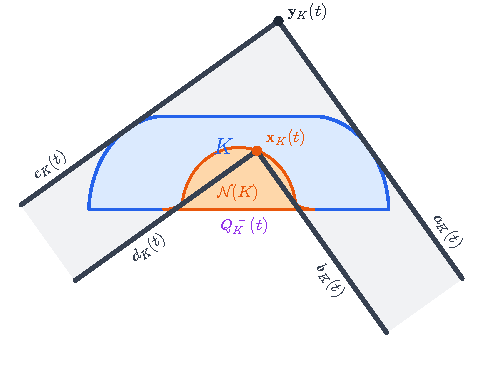
\includegraphics[width=0.74\linewidth]{figures/fig-cap}
\caption{A cap, its niche and a supporting hallway: Gerver's cap $K=\KG$ (blue), its niche $\cN(K)$ (orange), and the
supporting hallway $L_K(t)$ at $t=0.62$ (grey), whose outer walls $a_K(t)$ and $c_K(t)$ touch $K$ and meet at the outer
corner $\yy_K(t)$, and whose inner walls $b_K(t)$ and $d_K(t)$ meet at the inner corner $\xx_K(t)$, on the boundary of the
niche. $Q^-_K(t)$ is the open quarter-plane below the inner corner; the niche is the union of these quarter-planes over
$t\in(0,\pi/2)$, cut at the $x$-axis.}
\label{fig:cap}
\end{figure}

\begin{fact}[monotone sofas and caps]\label{fact:monotone}
Let $\omega\in(0,\pi/2]$.
\begin{enumerate}[label=(\alph*)]
\item\label{fact:monotone:envelope} If $S$ is a moving sofa with rotation angle $\omega$ in standard
position, then $\cI(S)$ is a moving sofa with rotation angle $\omega$ in standard position and
$S\subset\cI(S)$. \baek{Thm.~2.3.2}
\item\label{fact:monotone:cap} For such an $S$, $K=\cC(S)$ is a cap with $h_K=h_S$ on $J_\omega$, and
$\cI(S)=K\setminus\cN(K)$. \baek{Lemma~2.3.5, Thm.~2.4.1, Thm.~2.4.2}
\item\label{fact:monotone:area} If $T$ is a monotone sofa with rotation angle $\omega$ and $K=\cC(T)$,
then $T=K\setminus\cN(K)$, $\cN(K)\subset K$ and $\abs T=\cA_\omega(K)$. \baek{Thm.~2.4.3, Thm.~2.5.9, Thm.~2.5.10}
\item\label{fact:monotone:mirror} If $K$ is a cap, so is $K^{\mir}$, with $h_{K^{\mir}}(t)=h_K(\omega+\pi/2-t)$,
$\cN(K^{\mir})=M_\omega(\cN(K))$, $\cA_\omega(K^{\mir})=\cA_\omega(K)$ and
$\sigma_{K^{\mir}}(E)=\sigma_K(\omega+\pi/2-E)$ for Borel sets $E$. \baek{Prop.~2.5.4}
\end{enumerate}
\end{fact}

Three places need a remark. The proof of \ref{fact:monotone:envelope} uses Def.~2.3.9, which defines the left and the right side of a line
for lines not parallel to the $y$-axis, where it needs the $x$-axis (E1). In \ref{fact:monotone:cap}, the union over $t\in[0,\omega]$ in
Thm.~2.4.2 and the union over $(0,\omega)$ in the definition of the niche agree after intersection with $F_\omega$, and $\cC(S)$ is bounded also for $\omega=\pi/2$, which Baek does not show (E2). In
\ref{fact:monotone:mirror}, Prop.~2.5.4 prints $?_{K^{\mir}}(t)=M_\omega(?_K(\omega-t))$ for each of the walls $a,b,c,d$ and the ends $W,Z$, whereas $M_\omega$
exchanges $a\leftrightarrow c$, $b\leftrightarrow d$ and $W\leftrightarrow Z$, and the identity for the vertices has $K^{\mir}$ in place of $K$ on
the right (E3); \ref{fact:monotone:mirror} uses none of this.

Two more facts about caps are used without proof in Baek's \baek{Lemma~2.5.6}, \baek{Lemma~3.4.8} and \baek{Thm.~2.5.8} (E4): that $O$ and $o_\omega$ lie in every cap if $\omega<\pi/2$
(the statement about $o_\omega$ is not in the audit), and where the ends of the \emph{upper boundary} $\bigcup_{t\in[0,\omega+\pi/2]}e_K(t)$ of a cap $K$ are. Here
$A_K^\pm(t)=v_K^\pm(t)$ and $C_K^\pm(t)=v_K^\pm(t+\pi/2)$ \baek{Def.~2.5.1, Def.~2.5.2}.

\begin{lemma}[every cap contains $O$ and $o_\omega$]\label{lem:contains}
If $\omega<\pi/2$, every cap $K\in\Kc_\omega$ contains $O$ and $o_\omega$; in particular $h_K\ge0$. For $\omega=\pi/2$ the origin need not lie in $K$ (take $K=[5,6]\times[0,1]$).
\end{lemma}

\begin{proof}
Let $q\in K\cap l(\pi/2,1)$ and $q'\in K\cap l(\omega,1)$. As $K\subset P_\omega$, $q=o_\omega-\lambda u_0$ and $q'=o_\omega-\mu v_\omega$ with $\lambda,\mu\ge0$.
For $s\in[0,\omega]$, $\ip{o_\omega}{u_s}=\ip{q'}{u_s}+\mu\sin(s-\omega)\le\ip{q'}{u_s}\le h_K(s)$, and for $s\in[\pi/2,\omega+\pi/2]$,
$\ip{o_\omega}{u_s}=\ip q{u_s}+\lambda\cos s\le\ip q{u_s}\le h_K(s)$. As $o_\omega\in F_\omega$, \eqref{eq:cap-fan} gives $o_\omega\in K$. Then $h_K(s)\ge\ip{o_\omega}{u_s}=c_\omega\cos s+\sin s=\sqrt{1+c_\omega^2}\,\sin\bigl(s+\tfrac\pi4-\tfrac\omega2\bigr)$, because
$c_\omega=\tan(\pi/4-\omega/2)$, and $0<s+\pi/4-\omega/2<\pi$ for $s\in J_\omega$, so $h_K\ge0$ on $J_\omega$. Hence $O\in F_\omega$ satisfies $\ip O{u_s}=0\le h_K(s)$ for
$s\in J_\omega$, and $O\in K$ by \eqref{eq:cap-fan}; and $h_K(s)\ge\ip O{u_s}=0$ for every $s$.
\end{proof}

\begin{lemma}[the ends of the upper boundary]\label{lem:ends}
For every cap $K\in\Kc_\omega$,
\begin{equation}\label{eq:ends}
  A_K^-(0)=(h_K(0),0)\quad\text{and}\quad C_K^+(\omega)=h_K(\omega+\pi/2)\,v_\omega ;
\end{equation}
they lie on $l(\pi/2,0)$ and on $l(\omega,0)$.
\end{lemma}

\begin{proof}
Let $q\in e_K(\omega+\pi/2)$ and $p=q-\ip q{u_\omega}u_\omega=h_K(\omega+\pi/2)v_\omega$. Since $\ip q{u_\omega}\ge0$ ($K\subset P_\omega$) and $\cos(s-\omega)\ge0$ for $s\in J_\omega$, we have
$\ip p{u_s}\le\ip q{u_s}\le h_K(s)$ for $s\in J_\omega$. Also $p\in F_\omega$, since $h_K(\omega+\pi/2)\ge0$ (\cref{lem:contains}; for $\omega=\pi/2$, $p_y=0$). So $p\in K$ by \eqref{eq:cap-fan}.
As $\ip\cdot{u_\omega}\ge0=\ip p{u_\omega}$ on $K$, $p$ is the point of $e_K(\omega+\pi/2)$ farthest in the direction $v_{\omega+\pi/2}=-u_\omega$, that is $p=C_K^+(\omega)$.
The mirror image $K^{\mir}$ is a cap (\cref{fact:monotone}\ref{fact:monotone:mirror}) with $h_{K^{\mir}}(\omega+\pi/2)=h_K(0)$, and $M_\omega$ maps $v_\omega$ to $u_0$ and reverses orientation, so that
$C^+_{K^{\mir}}(\omega)=h_K(0)v_\omega$ is mapped to the lower end $A_K^-(0)$ of $e_K(0)$, which is $(h_K(0),0)$.
\end{proof}

The next fact is the main theorem of \cite{Baek}, in the form for caps. It assembles Baek's
construction of a balanced maximum cap $K_\omega$ for every $\omega$ (\baek{Thm.~3.5.2, Thm.~3.5.4}), its
maximality (\baek{Thm.~3.5.5}), and the optimality of Gerver's sofa $\Gs$ (\baek{Thm.~1.1.1}), which is
recalled in \cref{sec:gerver}.

\begin{fact}[optimality]\label{fact:optimal}
Every moving sofa $S$ has $\abs S\le\abs\Gs$, and $\abs\Gs>11/5$. For every $\omega\in(0,\pi/2]$ and every
cap $K\in\Kc_\omega$, $\cA_\omega(K)\le\abs\Gs$.
\end{fact}

For the last claim, \baek{Thm.~3.5.6} gives a monotone sofa $S_\omega=K_\omega\setminus\cN(K_\omega)$ whose cap
$K_\omega$ satisfies $\cA_\omega(K)\le\cA_\omega(K_\omega)$ for every cap $K$ \baek{Thm.~3.5.5}, and
$\cA_\omega(K_\omega)=\abs{S_\omega}\le\abs\Gs$ by \baek{Thm.~1.1.1} and \cref{fact:monotone}\ref{fact:monotone:area}.

\subsection{Polygon caps}\label{sec:polygon}

Let $\omega\in(0,\pi/2]$. An \emph{angle set} is a finite nonempty $\Theta\subset(0,\omega)$, and
$\Theta^\diamond=\Theta\cup(\Theta+\pi/2)\cup\{\omega,\pi/2\}\subset(0,\pi)$ is its set of
\emph{defining normals}; the two normals $\omega$ and $\pi/2$, which carry the two strips of $P_\omega$,
are \emph{pinned}, the others \emph{floating}. A \emph{polygon cap} with angle set $\Theta$ is a cap
that is an intersection of closed half-planes with normal angles in
$\Theta^\diamond\cup\{\omega+\pi,3\pi/2\}$; they form the set $\Kc_\Theta\subset\Kc_\omega$. A polygon cap
is the intersection of its supporting half-planes $H_K(s)$ at these normal angles. For a cap $K$ put
\begin{align*}
  \cC_\Theta(K)&=P_\omega\cap\bigcap_{t\in\Theta}Q_K^+(t),\qquad
  \cN_\Theta(K)=F_\omega\cap\bigcup_{t\in\Theta}Q_K^-(t),\\
  \cA_\Theta(K)&=\abs{\cC_\Theta(K)}-\abs{\cN_\Theta(K)} .
\end{align*}
Here the \emph{fan} $F_\omega$, and not the parallelogram $P_\omega$, cuts the polygon niche: the
printed \baek{Def.~3.2.5} has $P_\omega$ and with it \baek{Prop.~3.3.5} and \baek{Lemma~3.4.2} are
false, whereas the results of \baek{Ch.~3} hold with $F_\omega$, as the formalization proves (E6).

\begin{fact}[the polygon bound]\label{fact:polygon}
For every cap $K$ and angle set $\Theta$, $\cC_\Theta(K)$ is a polygon cap that contains $K$ and has the
same support values as $K$ on $\Theta^\diamond$, and $\cC_\Theta(K)=K$ if $K\in\Kc_\Theta$;
$\cN_\Theta(K)=\cN_\Theta(\cC_\Theta(K))\subset\cN(K)$. Hence
$\cA_\omega(K)\le\cA_\Theta(K)=\cA_\Theta(\cC_\Theta(K))$, and $\cA_\Theta(K)=\abs K-\abs{\cN_\Theta(K)}$
for a polygon cap. \baek{Prop.~3.2.1, Prop.~3.2.2, Thm.~3.2.3}
\end{fact}

\begin{fact}[bounded width]\label{fact:width}
For $t\in(0,\omega)$ there is a constant $c_{\omega,t}$ such that every polygon cap $K$ with an angle set $\Theta\ni t$
and $\cA_\Theta(K)>0$ has width $h_K(0)+h_K(\pi)\le c_{\omega,t}$. \baek{Lemma~3.4.2}
\end{fact}

\runin{Sides of the polygon niche.} For a polygon cap $K$ with angle set $\Theta$, the boundary of
$F_\omega\setminus\cN_\Theta(K)$ consists of an open half-line, a polyline $\mathbf p_K$ from
$C_K^+(\omega)$ to $A_K^-(0)$ (see \eqref{eq:ends}), along which the abscissa increases and whose segments have normal angles in $\Theta^\diamond$,
and an open half-line \baek{Thm.~3.4.4}.
For $t\in\Theta^\diamond$ let $\tau_K(t)$ be the total length of the segments of $\mathbf p_K$ with normal
angle $t$, and $\sigma_K(t)=\abs{e_K(t)}$ the length of the edge of $K$ with normal angle $t$.
The following is about every polygon cap; maximality plays no role in it.

\begin{fact}[sides of the polygon niche]\label{fact:sides}
Let $K\in\Kc_\Theta$.
\begin{enumerate}[label=(\alph*)]
\item\label{fact:sides:wall} For $t\in\Theta$, $\Hone(\partial\cN_\Theta(K)\cap\vec b_K(t))=\tau_K(t)$ and
$\Hone(\partial\cN_\Theta(K)\cap\vec d_K(t))=\tau_K(t+\pi/2)$. \baek{Lemma~3.4.5\,(1)}
\item\label{fact:sides:floor} For $t\in\{\omega,\pi/2\}$, $\Hone(\cN_\Theta(K)\cap l(t,0))=\sigma_K(t+\pi)-\tau_K(t)$.
\baek{Lemma~3.4.5\,(2)}
\item\label{fact:sides:identity}
$\displaystyle\sum_{t\in\Theta^\diamond}\sin t\,\bigl(\sigma_K(t)-\tau_K(t)\bigr)=0$. \baek{Proof of Lemma~3.4.6}
\end{enumerate}
\end{fact}

Baek obtains \ref{fact:sides:identity} from the vector identity $\sum_t\tau_K(t)v_t=C_K^+(\omega)-A_K^-(0)=\sum_t\sigma_K(t)v_t$, by taking the inner product with $u_0$
(note $\ip{v_t}{u_0}=-\sin t$); the formalization proves \ref{fact:sides:identity} in this sine form, and of the vector identity only its $\sigma$ half.

\runin{Support values and first variations.} For $h:\Theta^\diamond\to\R$ let
\begin{align*}
  P_h&=\bigcap_{s\in\{\omega,\pi/2\}}\bigl(H_-(s,h(s))\cap H_+(s,h(s)-1)\bigr),\\
  \cC_\Theta(h)&=P_h\cap\bigcap_{s\in\Theta^\diamond\setminus\{\omega,\pi/2\}}H_-(s,h(s)),\\
  F_h&=\bigcap_{s\in\{\omega,\pi/2\}}H_+(s,h(s)-1),\\
  \cN_\Theta(h)&=F_h\cap\bigcup_{t\in\Theta}\bigl(H^\circ_-(t,h(t)-1)\cap H^\circ_-(t+\tfrac\pi2,h(t+\tfrac\pi2)-1)\bigr),
\end{align*}
and $\cA_\Theta(h)=\abs{\cC_\Theta(h)}-\abs{\cN_\Theta(h)}$ (\baek{Def.~3.3.3}). For a polygon cap $K$ and
$h=h_K|_{\Theta^\diamond}$ these are $K$, $\cN_\Theta(K)$ and $\cA_\Theta(K)$ (\baek{Prop.~3.3.4, Prop.~3.3.5}, with $F_\omega$, E6). For $\eps>0$ and
$t\in\Theta^\diamond$ let $h^{t,\eps}_K$ be $h_K$ with the value at $t$ replaced by $h_K(t)+\eps$.

\begin{fact}[pushing one side]\label{fact:push}
Let $K\in\Kc_\Theta$ and $t\in\Theta^\diamond$.
\begin{enumerate}[label=(\alph*)]
\item\label{fact:push:derivative} There are $\eps_0>0$ and $M\ge0$ such that for $0<\eps\le\eps_0$
\[
  \bigl\lvert\cA_\Theta(h^{t,\eps}_K)-\cA_\Theta(K)-(\sigma_K(t)-\tau_K(t))\eps\bigr\rvert\le M\eps^2 .
\]
\item\label{fact:push:translate} If $\sigma_K(t)>0$, then for small $\eps>0$ the set $\cC_\Theta(h^{t,\eps}_K)$ is a translate $C+v$
of a polygon cap $C\in\Kc_\Theta$.
\item\label{fact:push:area} If $\cC_\Theta(h^{t,\eps}_K)=C+v$ with $C\in\Kc_\Theta$, then $\cA_\Theta(h^{t,\eps}_K)\le\cA_\Theta(C)$.
\end{enumerate}
\baek{Lemma~3.4.7, Lemma~3.4.8, Prop.~3.3.7, Thm.~3.3.6}
\end{fact}

Part \ref{fact:push:derivative} rests on \baek{Thm.~3.1.2}, which needs the Nef polygon (a set obtained from finitely many half-planes by intersections, unions and
complements) to be bounded; every use is to bounded polygons (E5, and Section~4 of REPORT.md in~\cite{Companion}). In the proof of
\baek{Lemma~3.4.7} the sign of the change of $\abs{\cN_\Theta}$ is misprinted (E27).

\subsection{The injectivity condition and arm lengths}\label{sec:arms}

The rest of this section, and \cref{sec:injectivity,sec:equality}, concern caps with rotation angle $\pi/2$, and
$\cA=\cA_{\pi/2}$. For $K\in\Kc_{\pi/2}$ the \emph{arm lengths} are
\[
  f_K^\pm(t)=\ip{\yy_K(t)-A_K^\pm(t)}{v_t},\qquad g_K^\pm(t)=\ip{\yy_K(t)-C_K^\pm(t)}{u_t},
\]
with $\yy_K(t)=h_K(t)u_t+h_K(t+\pi/2)v_t$ the outer corner of the supporting hallway and
$A_K^\pm,C_K^\pm$ as in \eqref{eq:ends}. Thus $\yy_K(t)=A_K^\pm(t)+f_K^\pm(t)v_t=C_K^\pm(t)+g_K^\pm(t)u_t$: these are
the distances from the outer corner to the points where $K$ touches the two outer walls. They are
nonnegative, $g_K^-\le g_K^+$, and $f_K^\pm,g_K^\pm$ are at most the diameter of $K$, because
$A_K^\pm(t)-C_K^\pm(t)=g_K^\pm(t)u_t-f_K^\pm(t)v_t$ joins two points of $K$.

\begin{definition}[injectivity condition]\label{def:inj}
A cap $K\in\Kc_{\pi/2}$ satisfies the \emph{injectivity condition} if
\begin{enumerate}[label=(\arabic*),leftmargin=2.2em]
\item $\sigma_K$ has a density on $[0,\pi/2)$ and on $(\pi/2,\pi]$ (the top edge, at $\pi/2$, may carry an atom);
\item the inner corner $\xx_K$ is continuously differentiable on $[0,\pi/2]$;
\item $\ip{\xx_K'(t)}{u_t}<0<\ip{\xx_K'(t)}{v_t}$ for $0<t<\pi/2$.
\end{enumerate}
We write $\Ki$ for the set of caps in $\Kc_{\pi/2}$ that satisfy the injectivity condition and have
$\abs K\ge11/5$.
\end{definition}

Condition (3) implies that the inner corner moves strictly to the left, so the path of the inner corner has
no self-intersections. We use the following.

\begin{fact}[arms]\label{fact:arms}
Let $K\in\Kc_{\pi/2}$.
\begin{enumerate}[label=(\alph*)]
\item\label{fact:arms:deriv} For every $t$, $\xx_K$ has the right derivative
$-(f_K^+(t)-1)u_t+(g_K^+(t)-1)v_t$, and the left derivative given by the same formula with $f^-_K,g^-_K$.
\baek{Thm.~6.2.3}
\item\label{fact:arms:integral} $f_K^+(b)-f_K^+(a)=\int_a^bg_K^+-\sigma_K((a,b])$ for $0\le a\le b\le\pi/2$.
\baek{Thm.~6.2.5}
\item\label{fact:arms:mirror} For the reflection $K^{\mir}$ in $x\mapsto-x$, $f_{K^{\mir}}^\pm(t)=g_K^\mp(\pi/2-t)$ and
$g_{K^{\mir}}^\pm(t)=f_K^\mp(\pi/2-t)$. \baek{Prop.~6.2.2}
\item\label{fact:arms:regular} If $K$ satisfies (1), then $A_K^+=A_K^-$ and $f_K^+=f_K^-$ on $[0,\pi/2)$,
$C_K^+=C_K^-$ and $g_K^+=g_K^-$ on $(0,\pi/2]$. With $A_K=A_K^-$, $C_K=C_K^+$, $f_K=f_K^-$ and $g_K=g_K^+$ these four functions are continuous on
$[0,\pi/2]$; $f_K(0)=g_K(\pi/2)=1$, and $\xx_K'(t)=-(f_K(t)-1)u_t+(g_K(t)-1)v_t$. In particular (2) holds, and
(3) says that $f_K,g_K>1$ on $(0,\pi/2)$. \baek{Def.~6.4.1, Prop.~6.4.5, Prop.~6.4.6} The end values $f_K(0)=g_K(\pi/2)=1$ are not stated there (E17).
\end{enumerate}
\end{fact}

In \ref{fact:arms:mirror} the printed statement forgets that the reflection reverses the angle (E13); in \ref{fact:arms:deriv} the right derivative is called the left one, and the second display of the printed theorem is about the left derivative (E14).
Let
\[
  k_0(x)=\max\Bigl(\abs{x-1},\tfrac{\abs{x-1}+1}2\Bigr),\qquad m_0(x)=x-k_0(x) .
\]
The function $k_0$ is $1$-Lipschitz, and $m_0$ is nondecreasing, with $m_0(x)=\frac32x-1$ on $[0,1]$,
$m_0(x)=\frac x2$ on $[1,2]$ and $m_0(x)=1$ on $[2,\infty)$. For a continuous $f$ on $[0,\pi/2]$ let
$\mathcal Ff(x)=1+\int_0^xm_0(f(\pi/2-u))\dd u$, and let $f_0=0$, $f_{j+1}=\max(f_j,\mathcal Ff_j)$.

\begin{fact}[convergence of arms and the iteration]\label{fact:iteration}
\begin{enumerate}[label=(\alph*)]
\item\label{fact:iteration:arms} If polygon caps $K_n$ with rotation angle $\pi/2$ converge in $\dH$ to a cap $K\in\Kc_{\pi/2}$, then
$\int_0^{\pi/2}\abs{g_{K_n}^+-g_K^+}\to0$. \baek{Lemma~6.4.2}
\item\label{fact:iteration:eleven} $f_{11}(x)>1$ for $x\in(0,\pi/2]$. \baek{Lemma~6.5.5}, which is printed for $x\in(0,1]$ and used on $(0,\pi/2]$ (E17)
\end{enumerate}
\end{fact}

\subsection{Baek's upper bound}\label{sec:Q}

Let $\varphi=\varphi_G=0.03917\ldots$ be Gerver's angle (\cref{sec:gerver}), $\varphi^{\mathrm R}=\varphi$ and
$\varphi^{\mathrm L}=\pi/2-\varphi$. For $K\in\Kc_{\pi/2}$ let $H^{\mathrm b}_K(t)=\{\ip p{u_t}\ge h_K(t)-1\}$ and
$H^{\mathrm d}_K(t)=\{\ip p{v_t}\ge h_K(t+\pi/2)-1\}$ be the closed half-planes bounded by the inner walls $b_K(t)$ and $d_K(t)$, on
the side away from $Q^-_K(t)$, and
\[
  B_K=K\cap\bigcap_{t\in[\varphi^{\mathrm R},\pi/2]}H^{\mathrm b}_K(t),\qquad
  D_K=K\cap\bigcap_{t\in[0,\varphi^{\mathrm L}]}H^{\mathrm d}_K(t).
\]
Baek's upper bound is the functional $\cQ$ of \baek{Def.~8.2.2} on the set $\cT$ of triples $(K,B,D)$ of convex bodies with
$K\in\Ki$, $B,D\subset K$, $h_K(t)+h_B(\pi+t)\le1$ on $[\varphi^{\mathrm R},\pi/2]$ with equality at the
ends, and $h_K(\pi/2+t)+h_D(3\pi/2+t)\le1$ on $[0,\varphi^{\mathrm L}]$ with equality at the ends. The sets $\Ki$ and $\cT$ are closed under Minkowski combinations
$c_\lambda((K,B,D),(K',B',D'))=((1-\lambda)K+\lambda K',\dots)$. A functional on such a set is
\emph{convex-linear} if it commutes with $c_\lambda$, and \emph{convex} or \emph{concave} if it satisfies the
corresponding inequality for $c_\lambda$. The \emph{canonical triple} of $K\in\Ki$ is $\xi_K=(K,B_K,D_K)$.
For a convex body $K$, $a<b<a+\pi$, and a continuous curve $\mathbf z:[a,b]\to\R^2$ of bounded variation
with $\mathbf z(t)\in l_K(t)$, put
\[
  \varrho_{K,\mathbf z}(t)=\ip{\mathbf z(t)-v_K^+(t)}{v_t},\qquad
  \cM_K(a,b;\mathbf z)=\tfrac12\int_a^b\varrho_{K,\mathbf z}(t)^2\dd t .
\]
By Mamikon's theorem \baek{Thm.~7.4.1} (see \cite{Mnatsakanian97}), $\cM_K(a,b;\mathbf z)$ is the area
swept by the tangent segments from $v_K^+(t)$ to $\mathbf z(t)$; we use it only through the formula, which makes $\cM_K(a,b;\mathbf z)$ a convex function of $\varrho_{K,\mathbf z}$.
The curves that occur are the outer corner $\yy_K$ and the tangent line parametrizations
$\mathbf l_K^T(t)=v_K(t,T)$ for $T-\pi<t<T$ (the point where $l_K(t)$ meets $l_K(T)$) and $\mathbf l_K^T(T)=v_K^-(T)$.
Let $\cS_K,\cR_B,\cL_D$ be the \emph{Mamikon terms}
\begin{align*}
  \cS_K&=\cM_K(0,\varphi^{\mathrm R};\mathbf l_K^{\pi/2})+\cM_K(\varphi^{\mathrm R},\varphi^{\mathrm L};\yy_K)\\
  &\qquad+\cM_K(\varphi^{\mathrm L},\tfrac\pi2;\mathbf l_K^{\pi-\varphi})+\cM_K(\tfrac\pi2,\pi;\mathbf l_K^{\pi}),\\
  \cR_B&=\cM_B(\pi+\varphi^{\mathrm R},\tfrac{3\pi}2;\mathbf l_B^{3\pi/2}),\qquad
  \cL_D=\cM_D(\tfrac{3\pi}2,\tfrac{3\pi}2+\varphi^{\mathrm L};\mathbf l_D^{3\pi/2+\varphi^{\mathrm L}}).
\end{align*}
(In the third term $\pi/2+\varphi^{\mathrm L}=\pi-\varphi$.) The printed $\cR_B$ has $\pi/2+\varphi^{\mathrm R}$ in place of
$\pi+\varphi^{\mathrm R}$ (E27).

\begin{fact}[the upper bound]\label{fact:Q}
There is a functional $\cQ$ on $\cT$ such that:
\begin{enumerate}[label=(\alph*)]
\item\label{fact:Q:triple} $\xi_K\in\cT$ for $K\in\Ki$, and $\cA(K)\le\cQ(\xi_K)$. \baek{Thm.~8.1.8, Thm.~8.2.4}
\item\label{fact:Q:decomp} $\cQ(K,B,D)=\Lambda(K)-\cS_K-\cR_B-\cL_D$, where $\Lambda$ (Baek's $\cP_K+\cS_K$, \baek{Def.~8.3.4}) is
convex-linear on $\Ki$. For each of the four terms of $\cS_K$ (resp.\ for $\cR_B$, for $\cL_D$) the
curve $\mathbf z$ above is convex-linear in $K$ (resp.\ in $B$, in $D$), so that $\varrho(t)$ is convex-linear for every $t$, and each of the terms $\cM$, being $\frac12\int\varrho^2$,
is convex. \baek{Lemma~8.3.3, Lemma~8.3.4, Lemma~8.3.7, Thm.~8.3.1, Thm.~8.3.2, Thm.~7.1.2, Thm.~7.4.1}
\item\label{fact:Q:max} $\cQ\le\cQ(\xi_G)=\abs\Gs$ on $\cT$, where $\xi_G=\xi_{\KG}$ is the canonical triple of Gerver's cap.
\baek{Cor.~8.5.8, Thm.~8.4.6}
\end{enumerate}
\end{fact}

Part \ref{fact:Q:triple} is stated in \cite{Baek} with a proof that uses $\cN(K)\subset K$, which $\Ki$ does not
provide; the statement is true and has a proof that avoids it, which is in~\cite{Companion} (E21). Also \baek{Thm.~8.1.1} (convexity of $\Ki$) uses
the Brunn--Minkowski inequality, and it holds as stated.

\subsection{Gerver's sofa}\label{sec:gerver}

Seen from a sofa that turns clockwise by $t\in[0,\pi/2]$, the hallway occupies $\xx(t)+R_tL$; the curve
$\xx:[0,\pi/2]\to\R^2$ is the \emph{rotation path}. The largest set that moves along $\xx$ is its
\emph{shape}
\[
  \operatorname{shape}(\xx)=H_L\cap\bigcap_{t\in[0,\pi/2]}\bigl(\xx(t)+R_tL\bigr)\cap\bigl(\xx(\pi/2)+R_{\pi/2}V_L\bigr).
\]
\emph{Gerver's sofa} $\Gs$ is the shape of Romik's rotation path~\cite{Romik18}, which is glued from five
explicit curves, on $[0,\varphi],[\varphi,\theta],[\theta,\pi/2-\theta],[\pi/2-\theta,\pi/2-\varphi]$ and
$[\pi/2-\varphi,\pi/2]$, with $\varphi=0.03917\ldots$ and $\theta=0.68130\ldots$ (the formulas and Romik's equations
are in Appendix~\ref{app:gerver}). Write $t_0,\dots,t_5=0,\varphi,\theta,\pi/2-\theta,\pi/2-\varphi,\pi/2$,
$\alpha=\ip{\xx'}{u_t}$, $\beta=\ip{\xx'}{v_t}$, and
\[
  \bA=\xx+\alpha v_t+u_t,\quad \bB=\xx+\alpha v_t,\quad \bC=\xx-\beta u_t+v_t,\quad \bD=\xx-\beta u_t
\]
for the contact points of the sofa with the walls of the hallway.

\begin{fact}[Gerver's sofa]\label{fact:gerver}
\begin{enumerate}[label=(\alph*)]
\item\label{fact:gerver:def} Romik's equations have exactly one solution with $\varphi\in[0.039,0.04]$,
$\theta\in[0.68,0.69]$, so $\Gs$ is well defined, and $2.2192\le\abs\Gs\le2.2199$. (Romik asserts, without proof, the uniqueness for $0<\varphi<\theta<\pi/4$; uniqueness in this box
is proved in~\cite{Companion}.)
\item\label{fact:gerver:cap} $\Gs$ is a monotone sofa with rotation angle $\pi/2$. Its cap $\KG=\cC(\Gs)$
satisfies $\Gs=\KG\setminus\cN(\KG)$ and has $A_{\KG}=\bA$, $C_{\KG}=\bC$ and $\xx_{\KG}=\xx$ on $[0,\pi/2]$; and
$\KG$ satisfies the injectivity condition; as $\abs\KG\ge\abs\Gs>11/5$, $\KG\in\Ki$. \baek{Thm.~8.4.1\,(1), Thm.~6.1.2}
\item\label{fact:gerver:niche} Let $\Gamma=\bD([t_0,t_2])\cup\xx([t_1,t_4])\cup\bB([t_3,t_5])$. Then
$\bD(t_0)$ and $\bB(t_5)$ lie on the $x$-axis, $\bD(t_2)=\xx(t_4)$, $\bB(t_3)=\xx(t_1)$, the abscissa is
strictly increasing along $\bD$ and $\bB$ and strictly decreasing along $\xx$ on $(0,\pi/2)$,
at every point of $[t_0,t_1]$ and of $[t_1,t_2]$ the curve $\bD$ has a derivative within that interval that is a positive multiple of $u_t$, and at every point of $[t_3,t_4]$ and of $[t_4,t_5]$ the curve $\bB$ has a
derivative within that interval that is a negative multiple of $v_t$ (the derivatives are one-sided at the ends of the pieces, and jump at $t_1$ and $t_4$), and
\[
  \cN(\KG)=\{q:\ q_y\ge0,\ q_y<\gamma_y\text{ for some }\gamma\in\Gamma\text{ with }\gamma_x=q_x\}.
\]
\baek{Thm.~8.4.1\,(2)--(4)}
\end{enumerate}
\end{fact}

Baek states \baek{Thm.~8.4.1} without proof (his Remark~8.4.1: the properties are ``easy to verify
numerically''), and proves \baek{Thm.~6.1.2} by a misreading of a theorem of Gerver (E12, E24). Both
statements are true; the formalization proves them from Romik's equations by interval
arithmetic~\cite{Companion}. Baek's \baek{Thm.~8.4.1\,(2)} describes the niche as the region enclosed by $\bB$ reversed, $\xx|_{[t_1,t_4]}$, $\bD$ reversed and the segment of
the $x$-axis from $\bD(t_0)$ to $\bB(t_5)$. That open region omits the open segment of the $x$-axis between $\bD(t_0)$ and $\bB(t_5)$, which lies in $\cN(\KG)$ because $F_{\pi/2}$ is closed. Because of the monotonicity of the abscissa,
$\cN(\KG)$ is the set of points of the closed upper half-plane that lie strictly below the curve $\Gamma$, which is the identity in \ref{fact:gerver:niche}; this exact form is proved in~\cite{Companion}. We also use one
numerical fact that is not in~\cite{Baek}:

\begin{fact}[height of the rotation path]\label{fact:height}
$\xx(t)_y<1$ for every $t\in[0,\pi/2]$, and $\xx(t)_y>0$ for $t\in[t_1,t_4]$. In fact $\max_t\xx(t)_y=\xx(\pi/4)_y=0.66426\ldots$ and
$\xx(t_1)_y=\xx(t_4)_y=0.05518\ldots$, but we use only the two bounds, which the formalization proves by interval
arithmetic~\cite{Companion}: $\xx(t)_y\le0.9925$ on each phase, and $\xx_y>0$ on $[t_1,t_4]$.
\end{fact}
